\documentclass[a4paper,11pt,handout]{beamer}

%%%%%%%%%%%%%%%%%%%%%%%%%%%%%%%%%%%%%%%%%%%%%%%%%%%%%%%%
% Change to 0 to produce only slides without the notes,%
% to 1 to generate an A4 document with the notes.      %
%%%%%%%%%%%%%%%%%%%%%%%%%%%%%%%%%%%%%%%%%%%%%%%%%%%%%%%%
\def\includeNotes{1}
%%%%%%%%%%%%%%%%%%%%%%%%%%%%%%%%%%%%%%%%%%%%%%%%%%%%%%%%

\usetheme{Pittsburgh}
\usecolortheme{whale}
\usepackage{siunitx}
\usepackage{graphicx}
\usefonttheme[onlymath]{serif}

\setlength{\parskip}{1em}

\graphicspath{{fig/}}

\setbeameroption{hide notes}
\setbeamertemplate{note page}[plain]
\usepackage{pgfpages}

% Define a layout to include 2 slides per page
\makeatletter
\define@key{pgfpagesuselayoutoption}{horizontal shift}%
{\def\pgfpageoptionhshift{#1}}
\define@key{pgfpagesuselayoutoption}{vertical shift}%
{\def\pgfpageoptionvshift{#1}}
\makeatother
\pgfpagesdeclarelayout{2 on 1 shifted}
{
	\edef\pgfpageoptionheight{\the\paperwidth} % landscaped by default
	\edef\pgfpageoptionwidth{\the\paperheight}
	\def\pgfpageoptionborder{0pt}
	\def\pgfpageoptionfirstshipout{1}
	\def\pgfpageoptionhshift{0pt}
	\def\pgfpageoptionvshift{0pt}
}
{
	\pgfpagesphysicalpageoptions
	{%
		logical pages=2,%
		physical height=\pgfpageoptionheight,%
		physical width=\pgfpageoptionwidth,%
		current logical shipout=\pgfpageoptionfirstshipout%
	}
	% stack on top of one another
	\pgfpageslogicalpageoptions{1}
	{%
		border shrink=\pgfpageoptionborder,%
		border code=\pgfusepath{stroke},%
		resized width=\pgfphysicalwidth,%
		resized height=.5\pgfphysicalheight,%
		center=\pgfpoint{.5\pgfphysicalwidth+\pgfpageoptionhshift}%
		{.75\pgfphysicalheight+\pgfpageoptionvshift}%
	}%
	\pgfpageslogicalpageoptions{2}
	{%
		border shrink=\pgfpageoptionborder,%
		resized width=\pgfphysicalwidth,%
		resized height=.5\pgfphysicalheight,%
		center=\pgfpoint{.5\pgfphysicalwidth+\pgfpageoptionhshift}%
		{.25\pgfphysicalheight+\pgfpageoptionvshift}%
	}%
}

\usepackage{ifthen}
\ifthenelse{\equal{\includeNotes}{1}}{%
	\pgfpagesuselayout{2 on 1 shifted}[%
		a4paper,border shrink=10mm, horizontal shift=0cm]
	\setbeameroption{show notes}}{}%


%%%%%%%%%%%%%%%%%%%%%%%%%%%%%%%%%%%%%%%%%%%%%%%%%%%%%%%%%%%

\title{Green communications in 5G}
\author{Tim Van Den Driesschen\\Rodrigo Arias Mallo}
\institute{Universitat Politècnica de Catalunya}
\date{\today}

\begin{document}

\begin{frame}
	\titlepage
\end{frame}
\note{}
%%%%%%%%%%%%%%%%%%%%%%%%%%%%%%%%%%%%%%%%%%%%%%%%%%%%%%%%%%%
\begin{frame}
\frametitle{Introduction}
\begin{itemize}

\item In the next decade, the number of connected devices is expected to 
increase 100 times and the data volume by 1000 times

\item Operators are already facing significant power bills

\item Moving towards green communications is important both for 
\textbf{environmental} and \textbf{economic} reasons

\end{itemize}
\end{frame}
\note{
One of the big challenges is to meet future requirements and expectations in an affordable and sustainable way. Low energy consumption is the key to achieve this. Already today, the mobile operator’s energy bill is an increasing part of their OPEX (operational expenditure)

This is also important from a sustainability perspective; even though mobile communications today only contribute to a fraction of a percent of the global CO2 footprint [5], it is important to maintain or even reduce this in the future 5GrEEn [6] is a joint effort of partners tightly connected to the METIS project representing the telecom vendor Perspective.

This paper takes as a starting point the situation of today and tries to pinpoint important focus areas when designing an energy efficient 5G mobile network architecture. The outline is as follows: After a more in-depth discussion on major challenges for mobile networks in the future, the important focus areas and some potential solutions are outlined. Finally, a summary and concluding remarks are provided.
}
%%%%%%%%%%%%%%%%%%%%%%%%%%%%%%%%%%%%%%%%%%%%%%%%%%%%%%%%%%%
\begin{frame}
	\frametitle{Network planning and deployment}
\end{frame}
\note{%
Intro:

One of the big challenges is to meet future requirements and expectations in an affordable and sustainable way. Low energy consumption is the key to achieve this. Already today, the mobile operator’s energy bill is an increasing part of their OPEX (operational expenditure)

This is also important from a sustainability perspective; even though mobile communications today only contribute to a fraction of a percent of the global CO2 footprint [5], it is important to maintain or even reduce this in the future 5GrEEn [6] is a joint effort of partners tightly connected to the METIS project representing the telecom vendor Perspective.

This paper takes as a starting point the situation of today and tries to pinpoint important focus areas when designing an energy efficient 5G mobile network architecture. The outline is as follows: After a more in-depth discussion on major challenges for mobile networks in the future, the important focus areas and some potential solutions are outlined. Finally, a summary and concluding remarks are provided.

}
%%%%%%%%%%%%%%%%%%%%%%%%%%%%%%%%%%%%%%%%%%%%%%%%%%%%%%%%%%%

\begin{frame}
	\frametitle{Challenges}
\begin{itemize}
\item Data traffic Volumes
\item The number of connected devices
\item  Diverse requirements
\item  Energy consumption
\end{itemize}

\end{frame}
\note{
Challenges:
green design perspective will be discussed in the following subsections
}
%%%%%%%%%%%%%%%%%%%%%%%%%%%%%%%%%%%%%%%%%%%%%%%%%%%%%%%%%%%

\begin{frame}
	\frametitle{Data traffic Volumes}
    \begin{itemize}
\item Today: 2 billion mobile broadband subscriptions 
\item Exponential growth in the following years 
\item A factor of 1000x capacity demand in 2020 vs 2012
\item  
\end{itemize}
\end{frame}
\note{Data traffic volumes:
Today, there are over 2 billion mobile broadband subscriptions worldwide, a figure that has grown by 40 percent annually over the last six years.

Furthermore, forecasts predict that data traffic volumes will experience an exponential growth in the coming years [2], as illustrated in Fig. 1. For example, it can be seen that the data traffic volumes are expected to increase approximately 10
times between 2012 and 2018 Predictions are made that per-user data rates are expected to grow by a factor of up to 50-100; on the other hand, the density of mobile Internet users is expected to increase by a factor of up to 10, implying a factor of 1000x capacity demand in the 2020 time frame
Hence, it is obvious that mobile systems in the future need to be capable of delivering significantly more capacity than today. 

In fact, up to now mobile networks were dimensioned by taking into account the peak
capacity. With this approach, the exponential growth rate will imply a costly network deployment. Instead, evolved mobile networks should satisfy the increasing traffic demand by a flexible availability of capacity (in time and space) in order to sustain the data rate development that has been observed during recent decades}
%%%%%%%%%%%%%%%%%%%%%%%%%%%%%%%%%%%%%%%%%%%%%%%%%%%%%%%%%%%

\begin{frame}
	\frametitle{The number of connected devices}
        \begin{itemize}
\item Today:  7 billion mobile devices  
\item Future: Smart devices (smart grid, sensors and surveilence camera's) 
\item Internet of things (IoT)
\item  
\end{itemize}
\end{frame}
\note{
Today, there are almost 7 billion mobile subscriptions, and thereby wireless connected devices, worldwide.

However, in the future, this is predicted to change, as different kinds of machines such as smart grid devices, sensors and surveillance cameras will be connected to the networks. 

This is usually referred to as Internet-of-things [3] or machine-to-machine (M2M)
communication, and means that everything that can benefit from a wireless connection will have a wireless connection
}
%%%%%%%%%%%%%%%%%%%%%%%%%%%%%%%%%%%%%%%%%%%%%%%%%%%%%%%%%%%
\begin{frame}
	\frametitle{Diverse requirements}
            \begin{itemize}
\item Different applications of 5G
\item Low latency 
\item Different data sizes
\item  
\end{itemize}
\end{frame}
\note{
Challenges:
green design perspective will be discussed in the following subsections


}
%%%%%%%%%%%%%%%%%%%%%%%%%%%%%%%%%%%%%%%%%%%%%%%%%%%%%%%%%%%
\begin{frame}
	\frametitle{Challenges}
\end{frame}
\note{
Challenges:
green design perspective will be discussed in the following subsections


}
%%%%%%%%%%%%%%%%%%%%%%%%%%%%%%%%%%%%%%%%%%%%%%%%%%%%%%%%%%%
\begin{frame}
	\frametitle{Challenges}
\end{frame}
\note{
Challenges:
green design perspective will be discussed in the following subsections


}
%%%%%%%%%%%%%%%%%%%%%%%%%%%%%%%%%%%%%%%%%%%%%%%%%%%%%%%%%%%
\begin{frame}
	\frametitle{Challenges}
\end{frame}
\note{
Challenges:
green design perspective will be discussed in the following subsections


}
%%%%%%%%%%%%%%%%%%%%%%%%%%%%%%%%%%%%%%%%%%%%%%%%%%%%%%%%%%%
\begin{frame}
	\frametitle{Challenges}
\end{frame}
\note{
Challenges:
green design perspective will be discussed in the following subsections


}
%%%%%%%%%%%%%%%%%%%%%%%%%%%%%%%%%%%%%%%%%%%%%%%%%%%%%%%%%%%
\begin{frame}
	\frametitle{Challenges}
\end{frame}
\note{
Challenges:
green design perspective will be discussed in the following subsections


}
%%%%%%%%%%%%%%%%%%%%%%%%%%%%%%%%%%%%%%%%%%%%%%%%%%%%%%%%%%%
\begin{frame}
	\frametitle{Challenges}
\end{frame}
\note{
Challenges:
green design perspective will be discussed in the following subsections


}
%%%%%%%%%%%%%%%%%%%%%%%%%%%%%%%%%%%%%%%%%%%%%%%%%%%%%%%%%%%
\begin{frame}
\frametitle{Reducing power consumption [181]}
	\begin{center}
	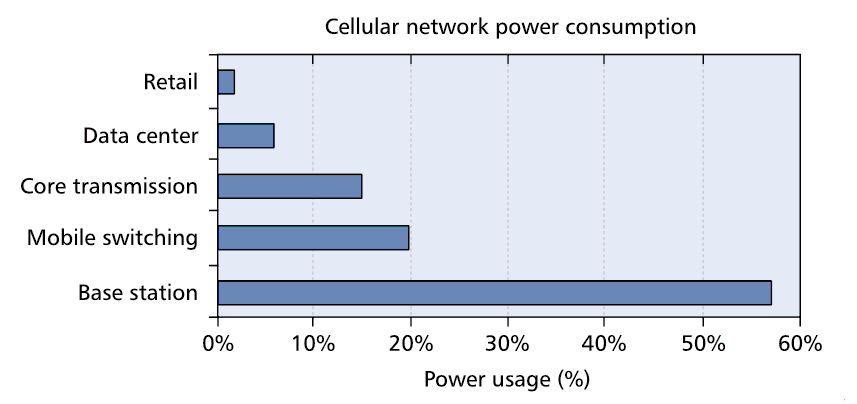
\includegraphics[scale=1]{consumption.png}
	\end{center}

\begin{itemize}

	\item The base station is the most power intensive element (more than 50\%).
	\item Also the usual lifetime is around 10--15 years, while smartphones is only 2.
	\item By reducing the power consumption of the largest element, the whole 
	consumption is reduced.

\end{itemize}
\end{frame}
\note{

}
%%%%%%%%%%%%%%%%%%%%%%%%%%%%%%%%%%%%%%%%%%%%%%%%%%%%%%%%%%%
\begin{frame}
\frametitle{Harvesting renewable energy resources}
In order to power the Base Stations (BS), energy can be obtained from renewable 
sources:

\begin{itemize}
\item Natural sources: Sun, wind, vibration
\item External: Batteries, fuel cells
\end{itemize}
\end{frame}
\note{%
Solar energy has been studied in UK cities, in order to power BS installed in 
road lamps, with a solar panel on top [175]. It has been observed that it can 
run fully autonomous, with the exception of the January month, where external 
power was needed.

Other sources of energy may not be so profitable, as sun is the source with the
highest amount of power, about \SI{100}{\milli\watt\per\centi\meter\squared}, 
followed by the wind with \SI{12}{\milli\watt\per\centi\meter\squared}.
}
%%%%%%%%%%%%%%%%%%%%%%%%%%%%%%%%%%%%%%%%%%%%%%%%%%%%%%%%%%%
\begin{frame}
	\frametitle{User-centric designs}
\end{frame}
\note{}
%%%%%%%%%%%%%%%%%%%%%%%%%%%%%%%%%%%%%%%%%%%%%%%%%%%%%%%%%%%
\begin{frame}
	\frametitle{Smaller frame overhead %
		\footnote{Following [178] paper in depth: Uplink Contention Based Multiple 
		Access for 5G Cellular IoT}%
	}

	\begin{itemize}
		\item Bursty traffic cause devices to change state between idle and 
		connected with the associate \textbf{power consumption}
		\item Significant \textbf{overhead} with small packets
		\item Contention based method have been proposed
		\end{itemize}
\end{frame}
\note{Expand based on reference 178}
%%%%%%%%%%%%%%%%%%%%%%%%%%%%%%%%%%%%%%%%%%%%%%%%%%%%%%%%%%%
\begin{frame}
	\frametitle{Uplink contention based methods}


	\begin{center}
	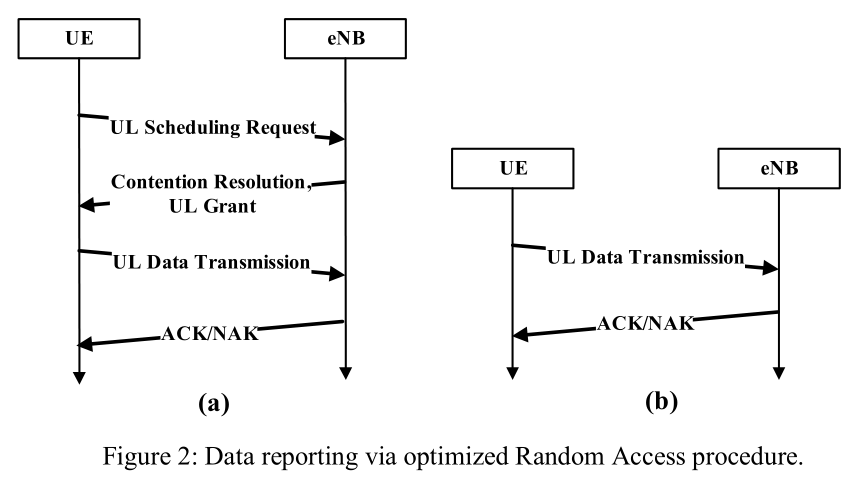
\includegraphics[scale=0.3]{uc.png}
	\end{center}

	\begin{itemize}
		\item Small signalling payload
		\item Direct small data packet
	\end{itemize}
\end{frame}
\note{}
%%%%%%%%%%%%%%%%%%%%%%%%%%%%%%%%%%%%%%%%%%%%%%%%%%%%%%%%%%%
\begin{frame}
	\frametitle{Results of simulation}

	\begin{center}
	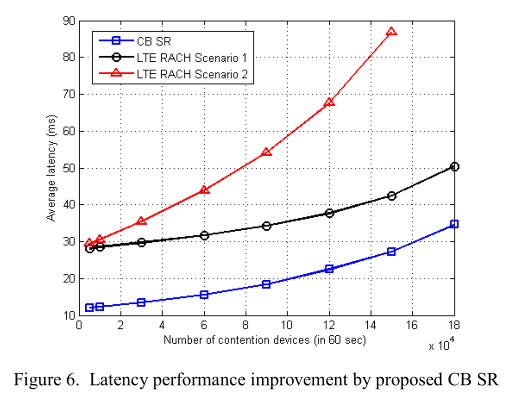
\includegraphics[scale=0.4]{cb-latency.png}
	\end{center}

\end{frame}
\note{}
%%%%%%%%%%%%%%%%%%%%%%%%%%%%%%%%%%%%%%%%%%%%%%%%%%%%%%%%%%%
\begin{frame}
\frametitle{Open problems}

\begin{itemize}
\item Power control: max power BS, sunlight.
\item Energy efficient hardware: transceivers
\item Energy efficient network architecture: SDN, NFV, data/control plane
\item New battery technologies: sugar bio-batteries%
\footnote{Following [183] paper in depth: \textsl{A high-energy-density sugar 
biobattery based on a synthetic enzymatic pathway}}, photo-MFC
\end{itemize}

\end{frame}
\note{
There are some challenges to be resolved.
\begin{itemize}
	\item Power control
	\begin{itemize}
		\item In multi-tiered networks, the user is not connected to the BS with 
		maximum power.
		\item Solar and wind energy harvesting can be unfeasible in dense localities 
		and where sunlight is not available.
	\end{itemize}
	\item Energy efficient hardware
	\begin{itemize}
		\item Current transceivers are energy costly, as they are designed for good 
		throughput.
	\end{itemize}
	\item Energy efficient network architecture
	\begin{itemize}
		\item Multiple technologies as MIMO, SDN, NFV, D2D, cloud computing...
		\item Separation of control and data planes
		\end{itemize}
	\item New battery technologies: sugar bio-batteries, photo-MFC%
	\begin{itemize}
		\item Based on enzymes that extract energy from sugar, similar to humans.
		\item Moss can also be used to harvest solar power
		\item Still with a low efficiency to be used.
	\end{itemize}
\end{itemize}
}
%%%%%%%%%%%%%%%%%%%%%%%%%%%%%%%%%%%%%%%%%%%%%%%%%%%%%%%%%%%
\begin{frame}
\frametitle{Sugar bio-batteries [183]}

	\begin{center}
	
\includegraphics[scale=0.3]{trash.jpg}
	\end{center}

\begin{itemize}

	\item The typical density of energy of a Lithium cell is around 
	\SI{0.54}{\mega\joule\per\kilogram}

	\item But the combustion energy of glucose can release up to 
	\SI{15.5}{\mega\joule\per\kilogram}

	\item Sugars are non toxic, safe and carbon neutral

\end{itemize}
\end{frame}
\note{
The energy per Kilogram stored in a lithium cell is about 2 orders of magnitude below the available energy in an equivalent sized glucose cell.


Those cells are able to work for long periods with a suitable flow of glucose-like input stream. The enzymes used for the transformation of sugar are non toxic, an easy to obtain, they don't need any exotic metal nor element.

Experiments with bio-batteries seem to have a suitable position as power cells.

The cells consist of some enzymes placed close to an electrode. A 

}
%%%%%%%%%%%%%%%%%%%%%%%%%%%%%%%%%%%%%%%%%%%%%%%%%%%%%%%%%%%
\begin{frame}
\frametitle{Sugar bio-batteries [183]}

\begin{itemize}

	\item Maltodextrin (food additive), produced from starch.
	\item Sugars are non toxic, safe and carbon neutral
	\item The lifetime of enzymes is very short (weeks)
	\item They have to be recharged regularly.

\end{itemize}
\end{frame}
\note{}
%%%%%%%%%%%%%%%%%%%%%%%%%%%%%%%%%%%%%%%%%%%%%%%%%%%%%%%%%%%



\begin{frame}
\frametitle{Energy efficiency metrics [179]}

\begin{itemize}

	\item We need some way to compare energy efficiency (EE), but which metric is 
more suitable?
	\item Output energy/input energy?
	\item Performance/energy consumption?
	\item What load should we use for the measurement?
	\item Accuracy?

\end{itemize}
\end{frame}
\note{
In order to obtain an meaningful comparison of different technologies used in 
electronic communications, some metrics should be established so we can compare 
the energy efficiency.

Some candidates as the output power by the input power are useful when we can 
measure the power, but some times other measurements are more interesting. For 
example if we look at a processing unit, we may be interested in the performance 
per watt.

The base stations can operate at different loads, and the metric should include 
information of the load to be compared. Also the accuracy of the metric should 
be taken into consideration, as it may include information of fluctuations when 
the system is under operation.

We will focus on the metrics used at different levels of abstraction, starting 
from the lowest part, the component level, to the uppermost, the network level.
}
%%%%%%%%%%%%%%%%%%%%%%%%%%%%%%%%%%%%%%%%%%%%%%%%%%%%%%%%%%%
\begin{frame}
\frametitle{EE at component level}

	\begin{figure}[h]
	\begin{center}
	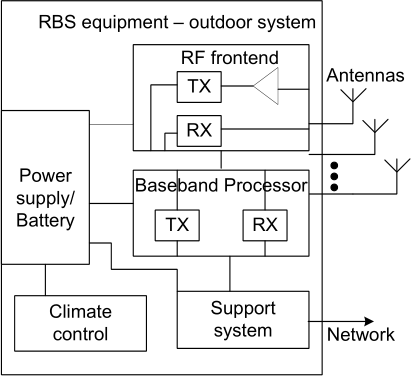
\includegraphics[scale=0.3]{ee-component.png}
	\end{center}
	\end{figure}

\begin{itemize}

	\item The components are analyzed by parts
	\item Example: The efficiency of the antenna as the input power that it 
receives compared with the irradiated power.
	\item On the baseband processor, EE is measured as performance per unit of 
energy consumption.
	\item For the power supply, output power/input power, often higher than 
85\%

\end{itemize}
\end{frame}
\note{
A general model is commonly used, as the one in the figure, to understand the 
different parts of a system. In each part we can identify and measure the 
efficiency based on specific metrics.

In the case of a radio base station, which may include one or more antennas, the 
efficiency can be expressed as the ratio of the radiated power $P_r$ to the 
input power $P_i$, $$ \eta = P_r / P_i$$

Whereas, in a baseband processor we are interested in the performance per watt, 
which can be measured by means of MFLOPS or MIPS which often can be expressed in 
equivalent MOPS (millions of operations per second).

The power supply is normally measured in terms of electrical efficiency, with 
the ration of output power by input power, often higher than 85\%.
}
%%%%%%%%%%%%%%%%%%%%%%%%%%%%%%%%%%%%%%%%%%%%%%%%%%%%%%%%%%%
\begin{frame}
\frametitle{EE at equipment level}

\begin{itemize}

	\item Power is computed by the average power level (high, med, low).
	\item Power supply correction factor and cooling factor.
	\item Energy consumption rating: Power/effective throughput.

\end{itemize}
\end{frame}
\note{

}
%%%%%%%%%%%%%%%%%%%%%%%%%%%%%%%%%%%%%%%%%%%%%%%%%%%%%%%%%%%
\begin{frame}
\frametitle{EE at network level}

\begin{itemize}

	\item Rural, cellular: Coverage area/average power consumption
	\item Urban: Subscribers/average power consumption
	\item Error correction: transmitter power/bit rate

\end{itemize}
\end{frame}
\note{}
%%%%%%%%%%%%%%%%%%%%%%%%%%%%%%%%%%%%%%%%%%%%%%%%%%%%%%%%%%%

\end{document}

